\documentclass[apacite, draftfirst, jou]{apa6}
\usepackage{amsmath}
\usepackage{float}
\usepackage{graphicx}
% \usepackage{color}
% \usepackage{relsize}
\setcounter{secnumdepth}{0}


\title{INSERT TITLE HERE}
\shorttitle{}

\threeauthors {Alex B. Carstenson} {Ryuka Ko} {Matthew J. Crossley}
\threeaffiliations {Stanford University} {RYUKA AFFILIATION} {Macquarie
  University}

\abstract{ABSTRACT GOES HERE.}

\rightheader{Draft}
\leftheader{Draft}

\begin{document}
\maketitle

\section{Introduction}

\section{Methods}
For the category-learning task, we used the procedure in Ashby et al. (2003),
which distinguished indicators in performance between rule-based versus
information-integration category learning. To generate our verbal and non-verbal
interference tasks, we referenced the method used in Gilbert et al. (2006),
which interleaved the interference and the main task to allow us to develop our
2-back matching interference paradigm.

\subsection{Participants}
122 participants were recruited from the University of California, Berkeley and
received course credit for participation. All the participants (mean age = 20.5
years) reported 20/20 vision or vision corrected to 20/20. Each individual
participated in only one of the six experiment conditions, resulting in the
following breakdown: rule-based/control (no interference), rule-based/verbal,
rule-based/spatial, information-integration/control (no interference),
information-integration/verbal, and information-integration/spatial. (From this
point forward, they will be referred to as RB-C, RB-V, RB-S, II-C, II-V, and
II-S, respectively).

\subsection{Stimuli Generation}
Category-learning stimuli: Every stimulus was a line that varied across two
dimensions – length and orientation. Two sets of 600 unique lines were generated
for each type of category structure using the procedure described in Ashby et
al. (2003). Each point in Figure 1 indicates the length and orientation of each
unique line. The rule-based category structure was unidimensional – it only
required the participant to attend to line length and ignore orientation
completely. Participants often described the categories as “one category was for
short lines and the other was for long lines.” On the other hand, the
information-integration category structure required participants to perceive
both dimensions. If a rule-based rule were used, it would only result in 70\%
accuracy at best. Unlike the rule-based structure, the information-integration
condition is difficult to describe verbally.

\subsection{Interference stimuli}
For the verbal interference task, the display presented a single word randomly
selected from this set: “thin,” “thick,” “straight,” “curved,” “solid,”
“narrow,” “slim,” “bent,” “wide,” “angled,” and “crooked.” These words were
specifically selected due to their association in typically being used to
describe types of lines. For the spatial (non-verbal) interference task, the
display showed a 5cm x 5cm grid in which 12 of the squares were black and 13
were white. A set of 15 unique displays were generated and randomly selected to
display.

\subsection{Procedure}
The experiment was run in a designated room on a computer. Participants were
given brief verbal instruction prior to the beginning of the experiment in which
the general format of the experiment was explained.

The experiment duration was about 60 minutes, with 12 blocks total, each block
consisting of 50 trials for a total of 600 trials. The participant would be
notified of each new block with a display that stated the Block number. The
category-learning stimuli and interference displays were interleaved (Figure 2).
A fixation marker was shown for 1.25 s. It was then followed by either a word
(verbal interference) or a grid (spatial interference) for 1.5 s. The
participant would then try to recall if the interference display was the same as
the interference display from two trials prior (two-back match). If it was the
same, the participant would press the space bar. No key press was required for a
non-matching interference.

For the interference task, the participants were urged to respond as quickly as
possible. No feedback was given to the participant regarding the accuracy of
their performance on the interference task. The fixation screen then reappeared
for another 1.25 s, followed by one of 600 randomly selected category-learning
lines. The line would be displayed until the participant pressed one of the two
category-learning keys. The category-learning keys were “D” and “K” on a
standard QWERTY keyboard. The keys were indicated with two different-colored
squares that covered the letter. Feedback was immediately displayed, with the
screen displaying either the word “Correct” or “Wrong” for 1 s. If they exceeded
the 5-second response requirement, “Please respond within 5 seconds” was
displayed on the screen for 1 s and the trial was discarded. Performance in the
interference task was emphasized over that in the categorization task.

Participants were also instructed that the response keys for the
category-learning task would switch for the last two blocks (Blocks 11 and 12).
Additionally, the response requirement for the category-learning task would
decrease from 5 sec to 1.5 sec to prevent participants from inhibiting their
initial response. If they exceeded the 1.5 sec response requirement, “Please
respond within 1.5 seconds” was displayed on the screen for 1 s and the trial
was discarded. Participants were assured that they would be informed of these
changes immediately before they occurred. “Respond quickly and the response
buttons will now be switched” was displayed on the monitor immediately prior to
the change. The interference task remained constant throughout the entire
experiment.

\section{Results}
\subsection{Dual-Task Performance}
Overall performance on the secondary task was good, with mean accuracies of 0.74
in the V-RB condition, 0.72 in the S-RB condition, 0.72 in the S-II condition,
and 0.80 in the V-II condition (see Fig. \ref{dt_accuracy}). A one-way ANOVA
with condition as a factor revealed that these differences were not significant
[$F(3, 106) = 2.03, p=0.11$].

\begin{figure}[h]
  \centering
  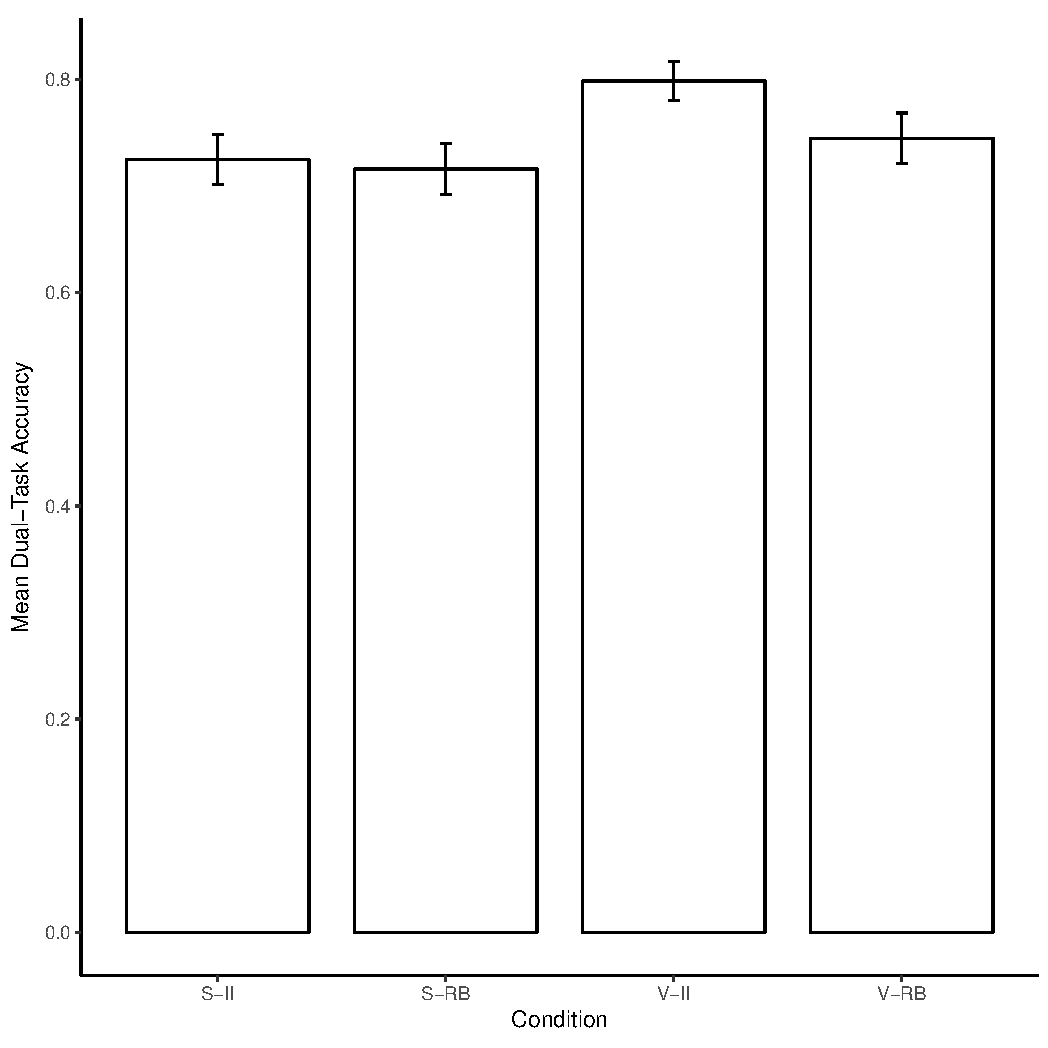
\includegraphics[width=0.5\textwidth]{../figs/dt_accuracy_bar.pdf}
  \caption{Mean dual-task accuracy across the entire experiment plotted
    separately for each condition. Error bars are SEM.}
  \label{dt_accuracy}
\end{figure}

\subsection{Category Learning Performance}
Performance during the training phase (i.e., every block up until the button
switch) of the expierment is shown in Fig. \ref{learning_curveas}. Within the II
conditions, there were no significant differences according to a one-way ANOVA
[$F(2,69) = 2.97, p = 0.06, Omega = 0.08$]. This ANOVA used condition as a
factor and the mean accuracy across the entire experiment for each participant
as the observations. However, independent samples t-tests revealed a significant
difference between the II-S and the II-V conditions [$t(29) = -2.56, p = 0.02, d
= 1.22$], but not between the other pairwise comparisons [II-S vs II-N: $t(31) =
-1.43, p = 0.16, d = 0.37$; II-V vs II-N: $t(45) = 1.29, p = 0.20, d = 0.25$].

Within the RB condtions, there were large significant differences according to
the same one-way ANOVA just described for the II condtions [$F(2,83) = 17.11, p
= 0.00, Omega = 0.29$]. Pairwise comparisons using independent samples t-tests
revealed that each RB condition is significantly different from every other RB
condition [RB-N vs RB-S: $t(39) = 3.16, p = 0.00, d = 1.59$; RB-N vs RB-V:
$t(58) = 7.05, p = 0.00, d = 6.54$; RB-S vs RB-V: $t(52) = 2.54, p = 0.01, d =
0.90$]. Visual inspection of Fig. \ref{learning_curves} clearly shows that these
differences show that both dual-tasks dignificantly impaired category learning
performance relative to the no dual-task control, and further shows that verbal
dual task caused much more interference than the spatial dual task.

\begin{figure}[h]
  \centering
  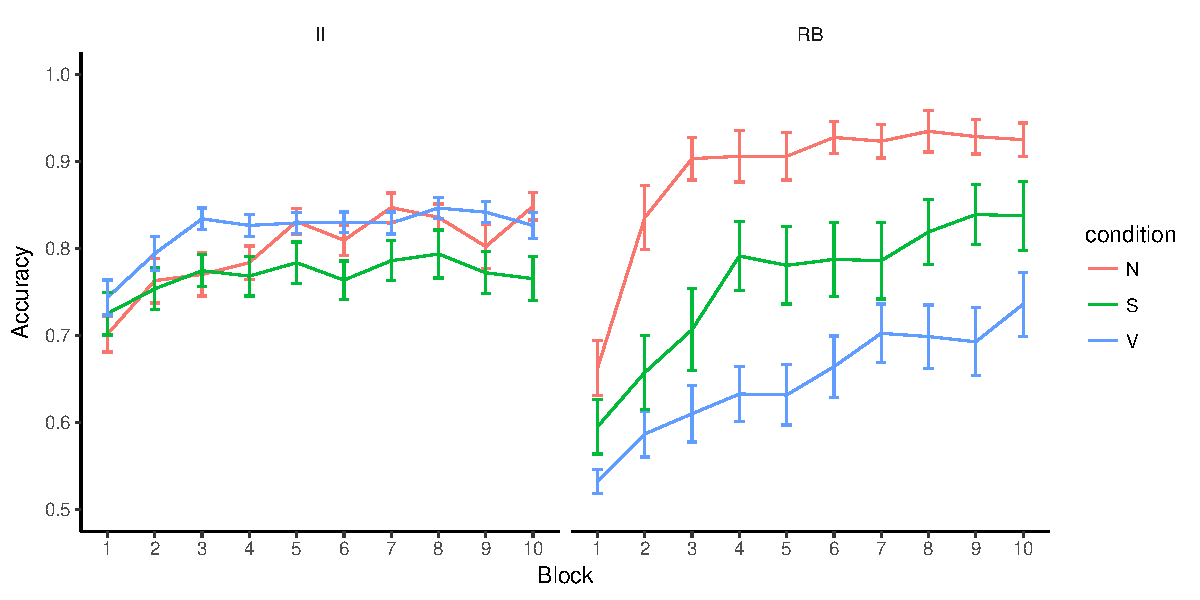
\includegraphics[width=0.5\textwidth]{../figs/learning_curves.pdf}
  \caption{Mean classification accuracy across participants computed sepatately
    for each condition and block of the experiment. Error bars are SEM.}
  \label{learning_curves}
\end{figure}

\subsection{Button Switch Performance}
Fig. \ref{bs_cost} shows the button-switch cost -- defined as mean block 10
accuracy minus the mean block 11 accuracy -- plotted separately for each
condition.

The button-switch cost was significant in the II-N [$t(24) = 2.60, p = 0.02, d =
1.38$] and II-V [$t(20) = -0.06, p = 0.95, d = 0.00$] conditions, but was not
significant in any other condition [II-S: $t(25) = 0.62, p = 0.54, d = 0.08$;
RB-N: $t(22) = 0.43, p = 0.67, d = 0.04$; RB-V: $t(36) = 1.66, p = 0.11, d =
0.46$; RB-S: $t(25) = 3.44, p = 0.00, d = 2.37$;].

The difference in button-switch cost was not significantly different betweeen
any pair of RB conditions [RB-S vs RB-V: $t(55) = -1.87, p = 0.07, d = 0.47$;
RB-N vs RB-S: $t(47) = -0.22, p = 0.82, d = 0.01$; RB-N vs RBV: $t(50) = -1.64,
p = 0.11, d = 0.38$].

The difference in button-switch cost in the II-S condition was significantly
different from the cost in the II-N condition [II-N vs II-S: $t(47) = 2.96, p =
0.00, d = 1.28$], but not significantly different than the cost in the II-V
condition, [II-V vs II-S: $t(42) = 1.98, p = 0.05, d = 0.61$] although this
latter difference was nearly significant. The difference in button-switch cost
between the II-V and the II-N condition was not signifiant [II-V vs ii-N: $t(44)
= -0.93, p = 0.36, d = 0.13$].

\begin{figure}[h]
  \centering
  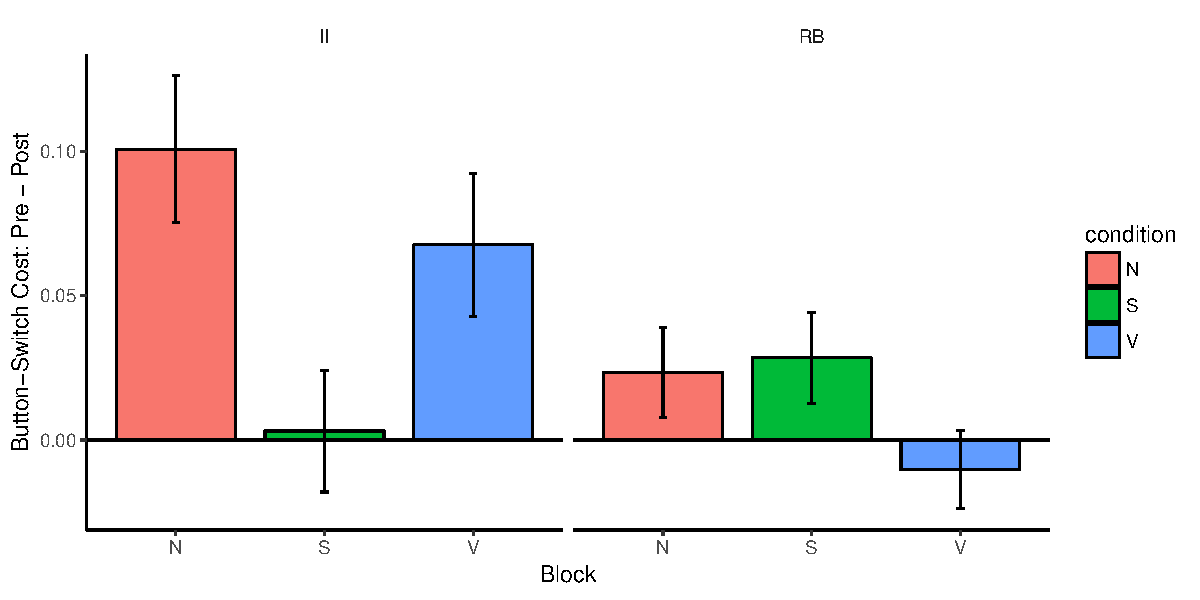
\includegraphics[width=0.5\textwidth]{../figs/bs_cost.pdf}
  \caption{Mean Accuracy difference between the last block of training and the
    first block of the button-switch (block 10 - block 11) plotted separately for
    each condition. Error bars are SEM.}
  \label{bs_cost}
\end{figure}

\section{Discussion}

\end{document}